%                                                              aanda.tex
% Transformer-based classification of TESS light curves
% Manuscript prepared with the A&A LaTeX class (aa.cls, v9.x)
%
% Compile with:  latexmk -pdf aanda.tex
%
% Class options that may be useful before submission:
%   \documentclass[referee]{aa}    % double-spaced referee version
%   \documentclass[longauth]{aa}   % long affiliation lists
%   \documentclass[rnote]{aa}      % research note
%   \documentclass[letter]{aa}     % letter
%-----------------------------------------------------------------------

\documentclass{aa}

\usepackage{graphicx}
\usepackage{txfonts}
\usepackage{amsmath}
\usepackage{booktabs}
\usepackage{siunitx}
\usepackage[colorlinks,citecolor=blue,linkcolor=blue,urlcolor=blue]{hyperref}

\graphicspath{{figures/}}

\sisetup{group-separator={\,},group-minimum-digits=4}

\begin{document}

    \title{Transformer-based classification of variable stars in TESS light curves}

    \subtitle{Multi-resolution views and fine-tuned time series foundation models}

    \author{
        A. Mateides\inst{1}
        \and
        P. \v{S}koda\inst{1,2}
    }

    \institute{Faculty of Information Technology, Czech Technical University in Prague,
        Th\'akurova 9, 160\,00 Prague 6, Czech Republic\\
        \and
        Astronomical Institute of the Czech Academy of Sciences,
        Fri\v{c}ova 298, 251\,65 Ond\v{r}ejov, Czech Republic
    }

    \date{Received ---; accepted ---}

% \abstract{}{}{}{}{}
% five mandatory {} tokens: context, aims, methods, results, conclusions

    \abstract
% context
    {Surveys such as OGLE, Kepler, ZTF, and TESS deliver light curves in numbers that make
    manual classification of variable stars impractical, and Gaia DR4 and PLATO will soon add more.}
% aims
    {We assess whether transformers are a viable backbone for variable-star classification
    from raw TESS photometry, and whether pretrained time series foundation models (TSFMs)
        and large language models (LLMs) can be fine-tuned to outperform both from-scratch
    transformers and a convolutional baseline.}
% methods
    {We used 3347 manually classified 2-min cadence light curves from the northern TESS
    continuous viewing zone, split into Task~A (variable versus
    non-variable) and Task~B (pulsating, rotating, eclipsing). Each light curve was cut
    into fixed-length segments, and each segment represented by four time-domain views at
    2, 8, 32, and 128\,min effective cadence, a phase-folded view, and scalar features. A
    multi-branch encoder processes each view in its own transformer branch using
    statistical patch embeddings, then fuses the branches linearly. Interchangeable
    backbones host transformers trained from scratch, a Chronos-2 TSFM, or a Qwen\,2.5
    0.5B LLM, the latter two fine-tuned with LoRA. Predictions are aggregated to the
    object (TIC) level by mean class probability.}
% results
    {Across 16 experiments, fine-tuned Chronos-2 was the only configuration beating the
    convolutional baseline on both tasks, reaching validation TIC-level macro
        $F_1$ of 0.926 (Task~A) and 0.950 (Task~B) against 0.906 and 0.923 for the baseline,
        and 0.893 and 0.880 on the test set. The Task~B loss is driven almost entirely by five
        atypical eclipsing systems. Multi-channel input and segmentation, not the backbone,
        account for most of the gain over single-view models.}
% conclusions
    {Fine-tuned TSFMs transfer effectively to stellar variability classification despite
    never having seen astronomical data, and the multi-resolution view representation is
    the decisive design choice. The pipeline processes $\sim$\,$10^6$ light curves per day
    on consumer hardware, making it applicable to survey-scale archives and to reducing
    exoplanet false positives.}

    \keywords{Methods: data analysis --
    Techniques: photometric --
    Stars: variables: general --
    Binaries: eclipsing --
    Surveys}

    \maketitle

%-----------------------------------------------------------------------


    \section{Introduction}
    \label{sec:intro}

    Variable stars underpin a large part of observational astrophysics. Their study
    produced the distance ladder that led to the discovery of the expansion of the Universe
    \citep{Hubble1929}, and the same photometric time series that reveal intrinsic
    variability are the raw material of transit-based exoplanet searches.

    Progress in photometric instrumentation has produced surveys of unprecedented volume:
    OGLE \citep{Udalski2008}, Kepler \citep{Borucki2010}, the Zwicky Transient Facility
    \citep{Bellm2019}, and the Transiting Exoplanet Survey Satellite
    \citep[TESS,][]{Ricker2014}. Two further large releases are imminent -- Gaia DR4
    \citep{Prusti2016} and the PLATO mission \citep{Rauer2025} -- and both will deliver
    light curves in quantities that rule out manual inspection.

    Machine learning has become the standard response. Convolutional networks in particular
    have repeatedly outperformed feature-engineered classifiers built on random forests or
    clustering. More recently, transformer architectures \citep{Vaswani2017} have become the
    dominant family for sequence modelling, and a parallel development -- large models
    pretrained on generic corpora and then adapted to a downstream task -- has proven
    effective in domains with little labelled data. Both developments are directly relevant
    here: labelled variable-star catalogues are small relative to the size of modern
    networks, while unlabelled light curves are abundant.

    In this work we ask two questions. First, can a transformer trained from scratch on a
    few thousand labelled TESS light curves compete with a convolutional baseline? Second,
    can large pretrained models -- a time series foundation model (TSFM) and a large
    language model (LLM), neither of which has ever seen astronomical data -- be fine-tuned
    into competitive classifiers of stellar variability? We answer both by evaluating 16
    configurations of a single modular architecture under an identical training and
    evaluation protocol.

    The paper is organised as follows. Section~\ref{sec:data} describes the TESS dataset and
    the two classification tasks. Section~\ref{sec:preproc} details the preprocessing
    pipeline, in particular the multi-resolution view representation that makes long light
    curves tractable for attention-based models. Section~\ref{sec:method} presents the
    architecture, the training objective, and the object-level evaluation protocol.
    Section~\ref{sec:results} reports the experiments, and Section~\ref{sec:discussion}
    discusses failure modes, throughput, and applicability. Section~\ref{sec:conclusions}
    concludes.

%-----------------------------------------------------------------------


    \section{Data}
    \label{sec:data}

    \subsection{TESS light curves}

    TESS \citep{Ricker2014} was launched by NASA in 2018. Although its primary mission is
    the detection of transiting exoplanets, it monitors every target that shows brightness
    variations, making it a rich source of variable-star photometry. Its four 16-megapixel
    wide-field cameras produce full-frame images from which individual targets are extracted
    as target pixel files; fluxes are then integrated to form time series, each identified by
    a unique TESS Input Catalogue number (TIC) \citep{TESSDataProducts}.

    We use light curves recorded at 2-min cadence. Their lengths vary considerably, from
    roughly \num{11000} to \num{216000} points. In raw form each record contains only a
    timestamp $t$ in Barycentric TESS Julian Date, a flux measurement $\Phi$, and its
    uncertainty $\Phi_{\mathrm{err}}$. Figure~\ref{fig:rawlc} shows a typical example,
    including the observing gap that occurs at each spacecraft perigee passage.

    \begin{figure}[!t]
        \centering
        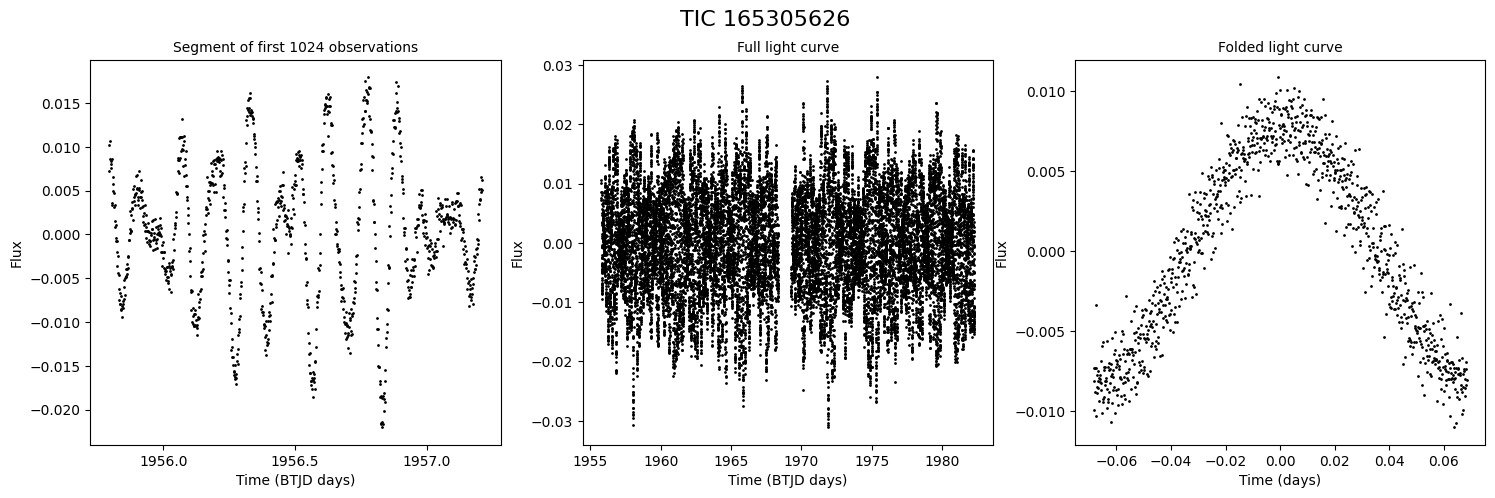
\includegraphics[width=\columnwidth]{05_raw_light_curve.png}
        \caption{Raw 2-min cadence light curve of a $\delta$\,Scuti star. Note the observing gap
        near the centre of the sector.}
        \label{fig:rawlc}
    \end{figure}

    \subsection{Labelled sample}

    Our sample is a cleaned subset of the manually labelled catalogue of periodic variable
    A--F stars in the northern TESS continuous viewing zone published by
    \citet{Skarka2022}, to which we refer for the full classification procedure.

    The catalogue contains 3402 light curves annotated with 49 distinct class labels, of
    which only 13 have more than ten members. We merged these into five superclasses.
    Objects carrying ambiguous multi-class annotations spanning different superclasses
    (e.g. ROTM/ELL) and extremely rare classes were discarded; this affected 55 objects and
    left \num{3347} light curves. Table~\ref{tab:classes} summarises the mapping.

    \begin{table}[!t]
        \caption{Label mapping from the original annotations of \citet{Skarka2022} to the five
        superclasses used in this work.}
        \label{tab:classes}
        \centering
        \small
        \begin{tabular}{llr r}
            \toprule
            Superclass               & Original labels & Count      & Total      \\
            \midrule
            Non-variable (N)         & NONE            & \num{1729} & \num{1729} \\
            \midrule
            Unspecified variable (U) & VAR             & 720        & 720        \\
            \midrule
            Pulsating (P)            & GDOR            & 206        &            \\
            & DSCT+GDOR       & 176        &            \\
            & GDOR+DSCT       & 86         &            \\
            & DSCT            & 67         & 535        \\
            \midrule
            Rotating (R)             & ROTS            & 175        &            \\
            & ROT             & 74         &            \\
            & ROTM            & 13         & 262        \\
            \midrule
            Eclipsing (E)            & EA              & 47         &            \\
            & ELL             & 24         &            \\
            & EW              & 17         &            \\
            & EB              & 13         & 101        \\
            \midrule
            \textbf{Total}           &                 &            & \num{3347} \\
            \bottomrule
        \end{tabular}
    \end{table}

    \subsection{Hierarchical task definition}

    Separating variables from non-variables and assigning a variability type to a confirmed
    variable are related but distinct problems, with very different class balance and very
    different decision boundaries. We therefore adopt a hierarchical formulation:

    \begin{description}
        \item[Task A] Binary classification: \emph{variable} (U, P, R, E merged) versus
        \emph{non-variable} (N). This task uses all \num{3347} objects and is close to
        balanced (\num{1729} vs \num{1618}).
        \item[Task B] Three-class classification of confirmed variables of known type:
        \emph{pulsating} (535), \emph{rotating} (262), \emph{eclipsing} (101), for a total
        of 898 objects. The unspecified-variable class is excluded, since it carries no
        type information.
    \end{description}

    Task~B is the harder problem: it has roughly a quarter of the objects of Task~A and a
    5:1 imbalance between its most and least populated classes.

%-----------------------------------------------------------------------


    \section{Preprocessing}
    \label{sec:preproc}

    Raw light curves cannot be fed directly to an attention-based model: they are far too
    long, they contain gaps, and their flux scales differ by orders of magnitude between
    targets. We describe the pipeline used to produce model inputs, including the steps that
    were evaluated and rejected.

    \subsection{Time standardisation and flux normalisation}

    Each light curve is shifted to a common origin, $t' = t - t_0$, so that all series start
    at $t'=0$. Fluxes are mapped to $[-1,1]$ by a modified min--max normalisation,
    \begin{equation}
        \Phi' = 2\,\frac{\Phi - \Phi_{\min}}{\Phi_{\max} - \Phi_{\min}} - 1 ,
    \end{equation}
    which centres the series on zero and thus reflects the physical behaviour of a flux
    oscillating about a mean level. Normalisation to $[0,1]$ gave statistically
    indistinguishable results. Because variability class is encoded mainly in light-curve
    morphology rather than amplitude, discarding the amplitude scale improves
    generalisation; the amplitude itself is retained separately as a scalar feature
    (Sect.~\ref{sec:scalars}).

    \subsection{Detrending}

    Detrending is routinely applied to remove instrumental drifts and low-frequency
    systematics,
    \begin{equation}
        \Phi' = \Phi - \Phi_{\mathrm{trend}} ,
    \end{equation}
    with $\Phi_{\mathrm{trend}}$ estimated by a running median, a Gaussian convolution, or a
    low-order polynomial fit. We evaluated all three with a range of window sizes and
    kernel widths. None improved classification performance over the untreated series.
    The reason is physical: rotational variables are defined precisely by the long-timescale
    modulation that these filters suppress. Detrending remains valuable for other tasks --
    eclipse searches in particular -- but was removed from our final pipeline.

    \subsection{Observing gaps}

    Invalid flux values (NaN, $\pm\infty$) are identified and encoded in a binary validity
    mask. The mask is applied inside the attention operation, so that invalid positions
    cannot contribute to any other token. When a CLS token is used for classification no
    further handling is needed; with mean pooling the mask must be applied a second time so
    that invalid tokens are excluded from the pooled representation.

    \subsection{Multiple time-domain views}
    \label{sec:views}

    The cost of self-attention grows quadratically with sequence length
    \citep{Vaswani2017}, which makes ingesting a full 2-min cadence sector -- $10^5$ points
    or more -- infeasible. Downsampling to a manageable length, on the other hand, destroys
    the short-period signal that distinguishes $\delta$\,Scuti pulsators.

    Our solution is to present the model with several views of the same interval at different
    temporal resolutions. Each view has a fixed length of 256 points, and is obtained by
    selecting a window at the start of the segment and mean-binning it to that length. We use
    four resolutions:

    \begin{itemize}
        \item 2\,min (native cadence, bin size 1),
        \item 8\,min (bin size 4),
        \item 32\,min (bin size 16),
        \item 128\,min (bin size 64).
    \end{itemize}

    A 128-min view of length 256 therefore covers $\left(128/2\right)\times 256 = \num{16384}$
    raw points, i.e. roughly 23\,d, while the 2-min view resolves individual pulsation
    cycles over the first $\sim$\,8.5\,h. Since all views start at the same point, the
    higher-resolution views are strict sub-intervals of the lower-resolution ones
    (Fig.~\ref{fig:views}). Together they span timescales from minutes to weeks at constant
    input length.

    \begin{figure}[!t]
        \centering
        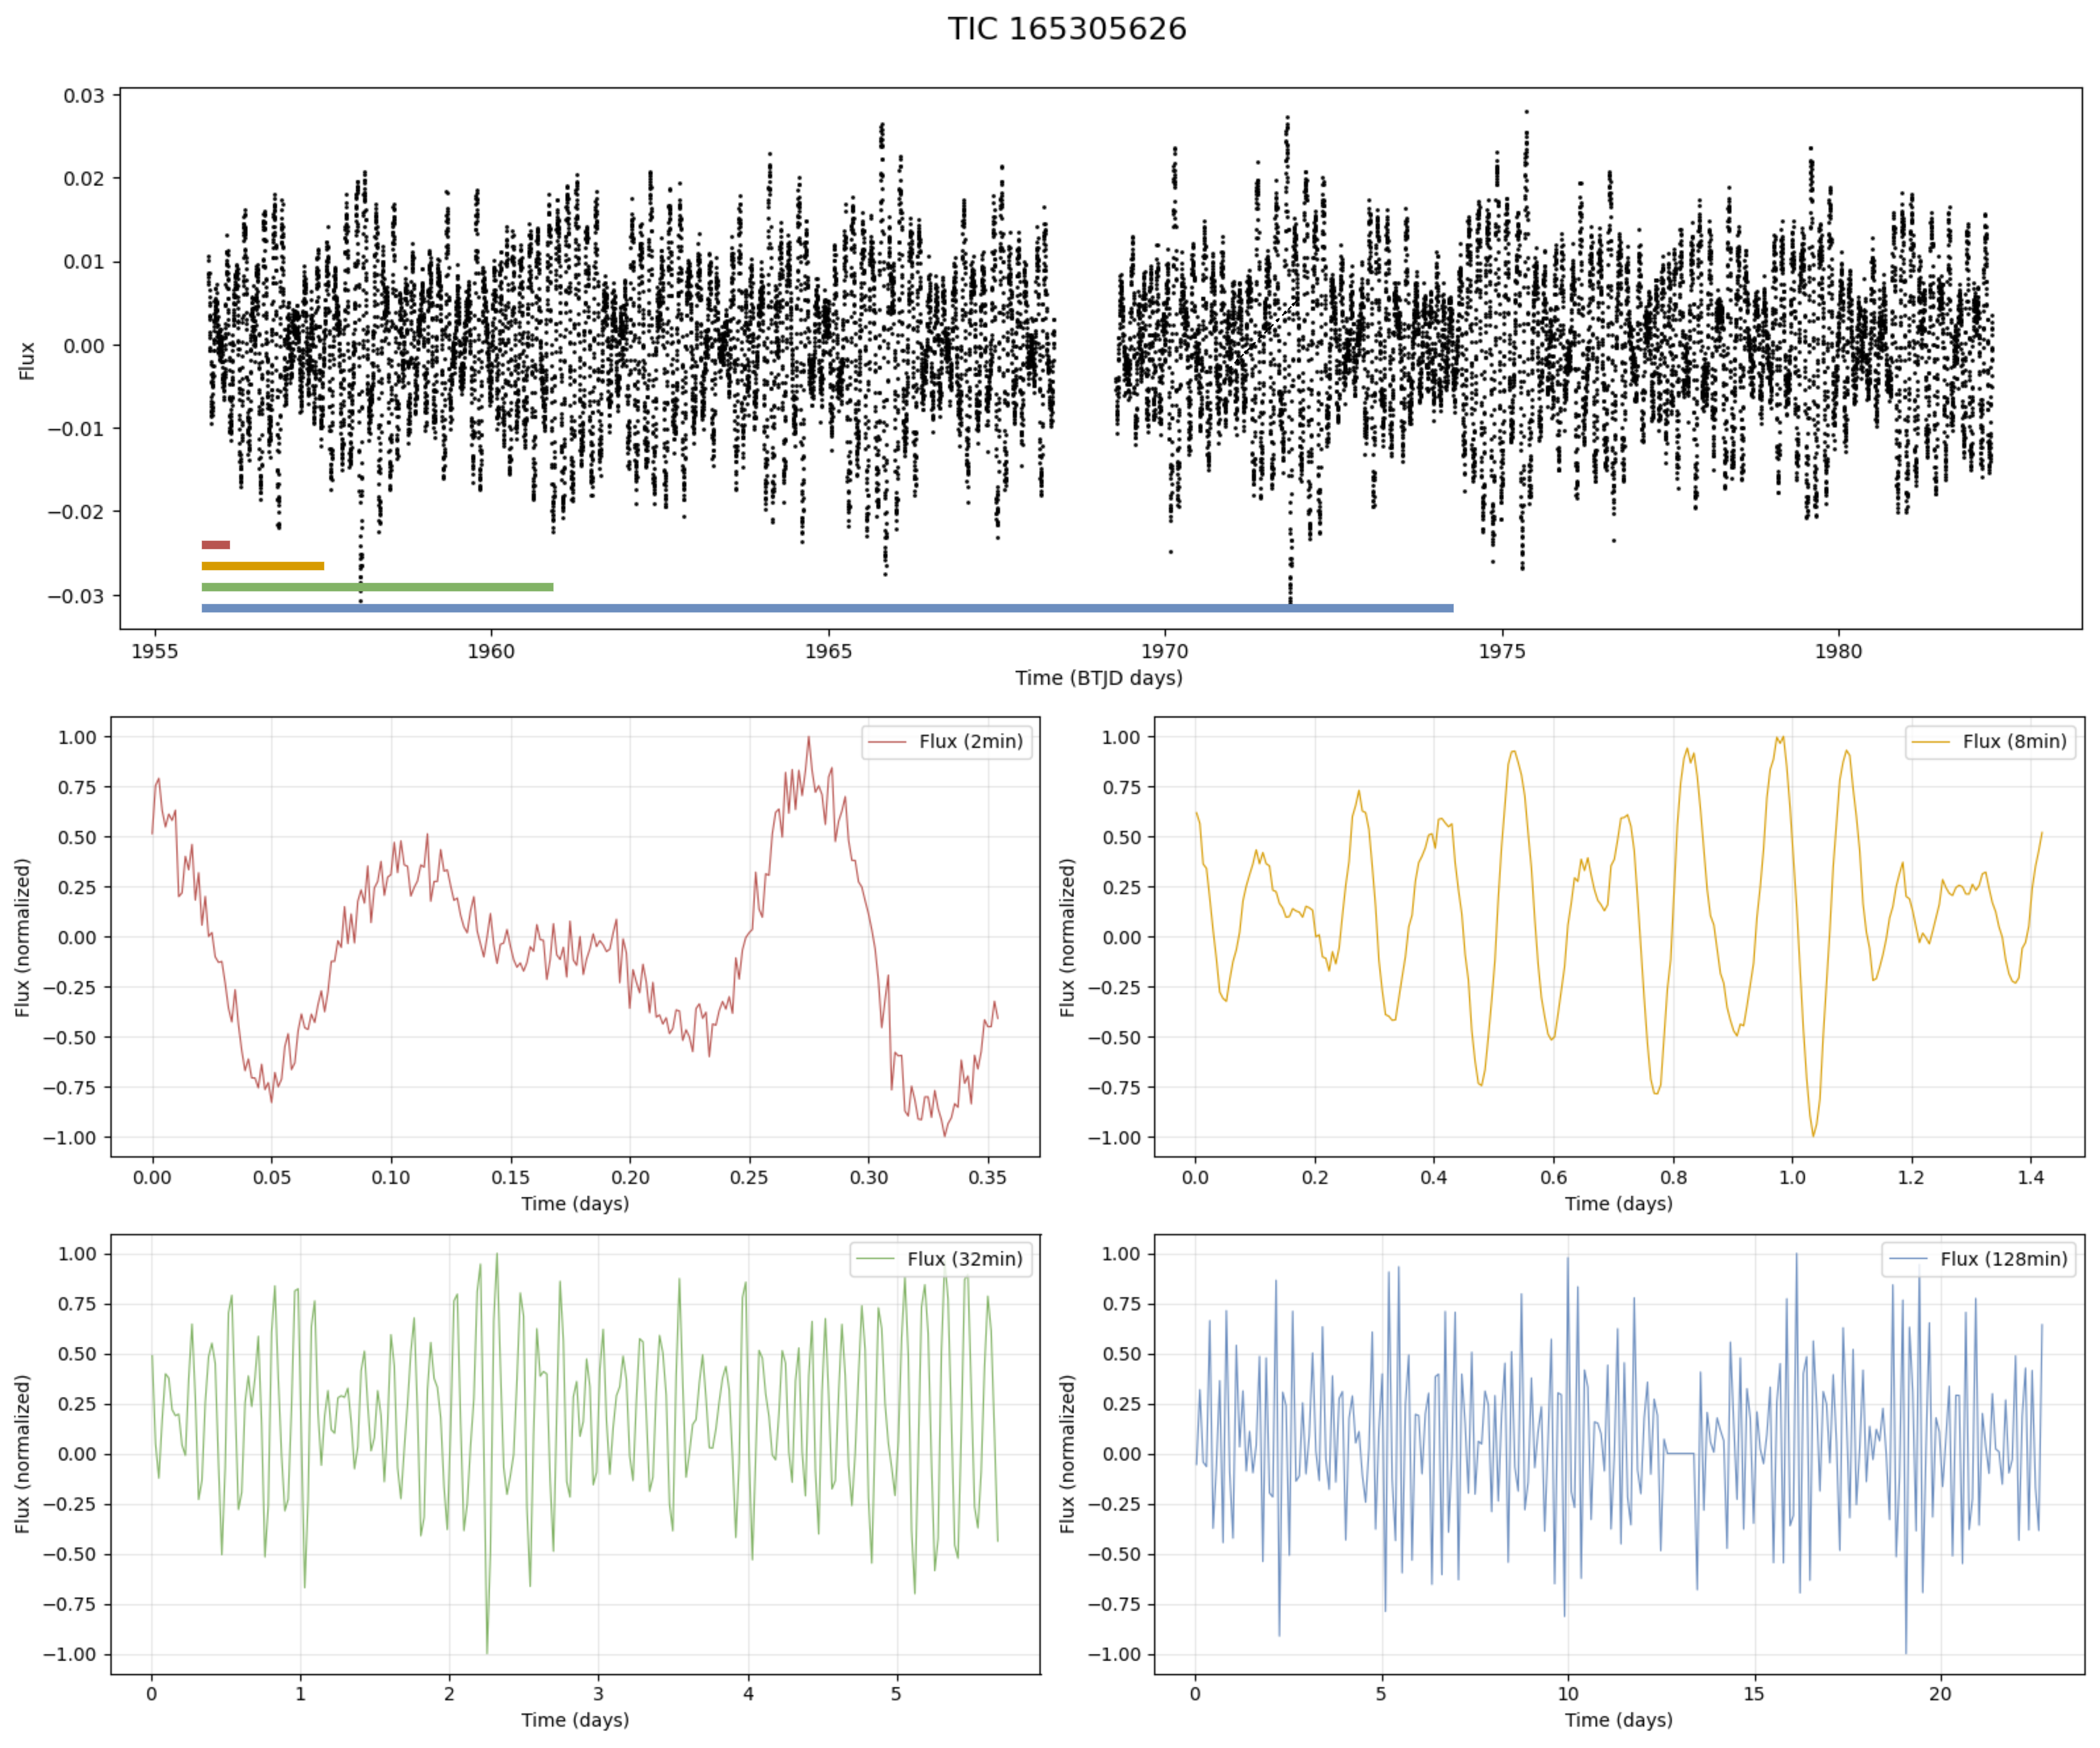
\includegraphics[width=\columnwidth]{light_curve_time_views.png}
        \caption{Four time-domain views of the light curve of a $\delta$\,Scuti star. Each view
        contains 256 points sampled at effective cadences of 2, 8, 32, and 128\,min. The coloured
        bars indicate the extent of each view within the original series.}
        \label{fig:views}
    \end{figure}

    \subsection{Segmentation}

    The labelled sample is small -- 898 objects with a specified variability type, only 101
    of them eclipsing -- which severely limits the capacity of network that can be trained.
    We therefore split each light curve into consecutive segments, each the length of the
    largest view window (\num{4096} raw points minimum, stride \num{4096}). Incomplete
    trailing segments are retained and masked. This yields \num{113355} training segments for
    Task~A and \num{30850} for Task~B (Table~\ref{tab:datasets}), more than an order of
    magnitude more samples than there are objects.

    Segmentation introduces three complications, all of which must be handled explicitly:

    \begin{itemize}
        \item \emph{Leakage.} Train/validation/test splits are made at the TIC level, so all
        segments of a given star fall in the same subset.
        \item \emph{Segment imbalance.} Objects yield different numbers of segments, so naive
        class weights are biased towards classes whose members happen to have longer
        light curves. This is corrected in the loss (Sect.~\ref{sec:loss}).
        \item \emph{Evaluation.} Segment-level metrics do not answer the scientific question.
        Predictions are aggregated to the object level (Sect.~\ref{sec:ticmetrics}).
    \end{itemize}

    \begin{table}[!t]
        \caption{Composition of the two task datasets after preprocessing.}
        \label{tab:datasets}
        \centering
        \small
        \begin{tabular}{llrr}
            \toprule
            Task & Class            & Objects    & Segments     \\
            \midrule
            A    & Non-variable (N) & \num{1729} & \num{57262}  \\
            & Variable (V)     & \num{1618} & \num{56093}  \\
            & \textbf{Total}   & \num{3347} & \num{113355} \\
            \midrule
            B    & Pulsating (P)    & 535        & \num{17868}  \\
            & Rotating (R)     & 262        & \num{9806}   \\
            & Eclipsing (E)    & 101        & \num{3176}   \\
            & \textbf{Total}   & 898        & \num{30850}  \\
            \bottomrule
        \end{tabular}
    \end{table}

    \subsection{Phase-folded view}

    A Lomb--Scargle periodogram \citep{Lomb1976,Scargle1982} is computed for each light
    curve, the dominant period is extracted, and the series is phase-folded on it and binned
    to the standard length of 256. This provides a fifth input channel in which periodic
    signals are coherently stacked, complementing the four time-domain views.

    \subsection{Scalar features}
    \label{sec:scalars}

    Three groups of scalar quantities are extracted and supplied through a separate branch:
    the pre-normalisation amplitude, which restores the physical scale removed by
    normalisation; the ten strongest periods identified in the periodogram; and their
    corresponding powers. These carry information that is difficult for a patch-based
    encoder to recover from a truncated view.

%-----------------------------------------------------------------------


    \section{Method}
    \label{sec:method}

    \subsection{Architecture}

    The classifier consists of six parallel branches feeding a linear fusion layer
    (Fig.~\ref{fig:arch}): five encoder-only transformer branches, one per input channel
    (four time-domain views plus the phase-folded view), and one multilayer-perceptron branch
    for the scalar features. Each branch can be enabled or disabled independently through the
    configuration file, which allows any subset of channels to be evaluated without code
    changes. The transformer blocks themselves are interchangeable, so the same architecture
    can host encoders trained from scratch or pretrained backbones.

    \begin{figure*}[!t]
        \centering
        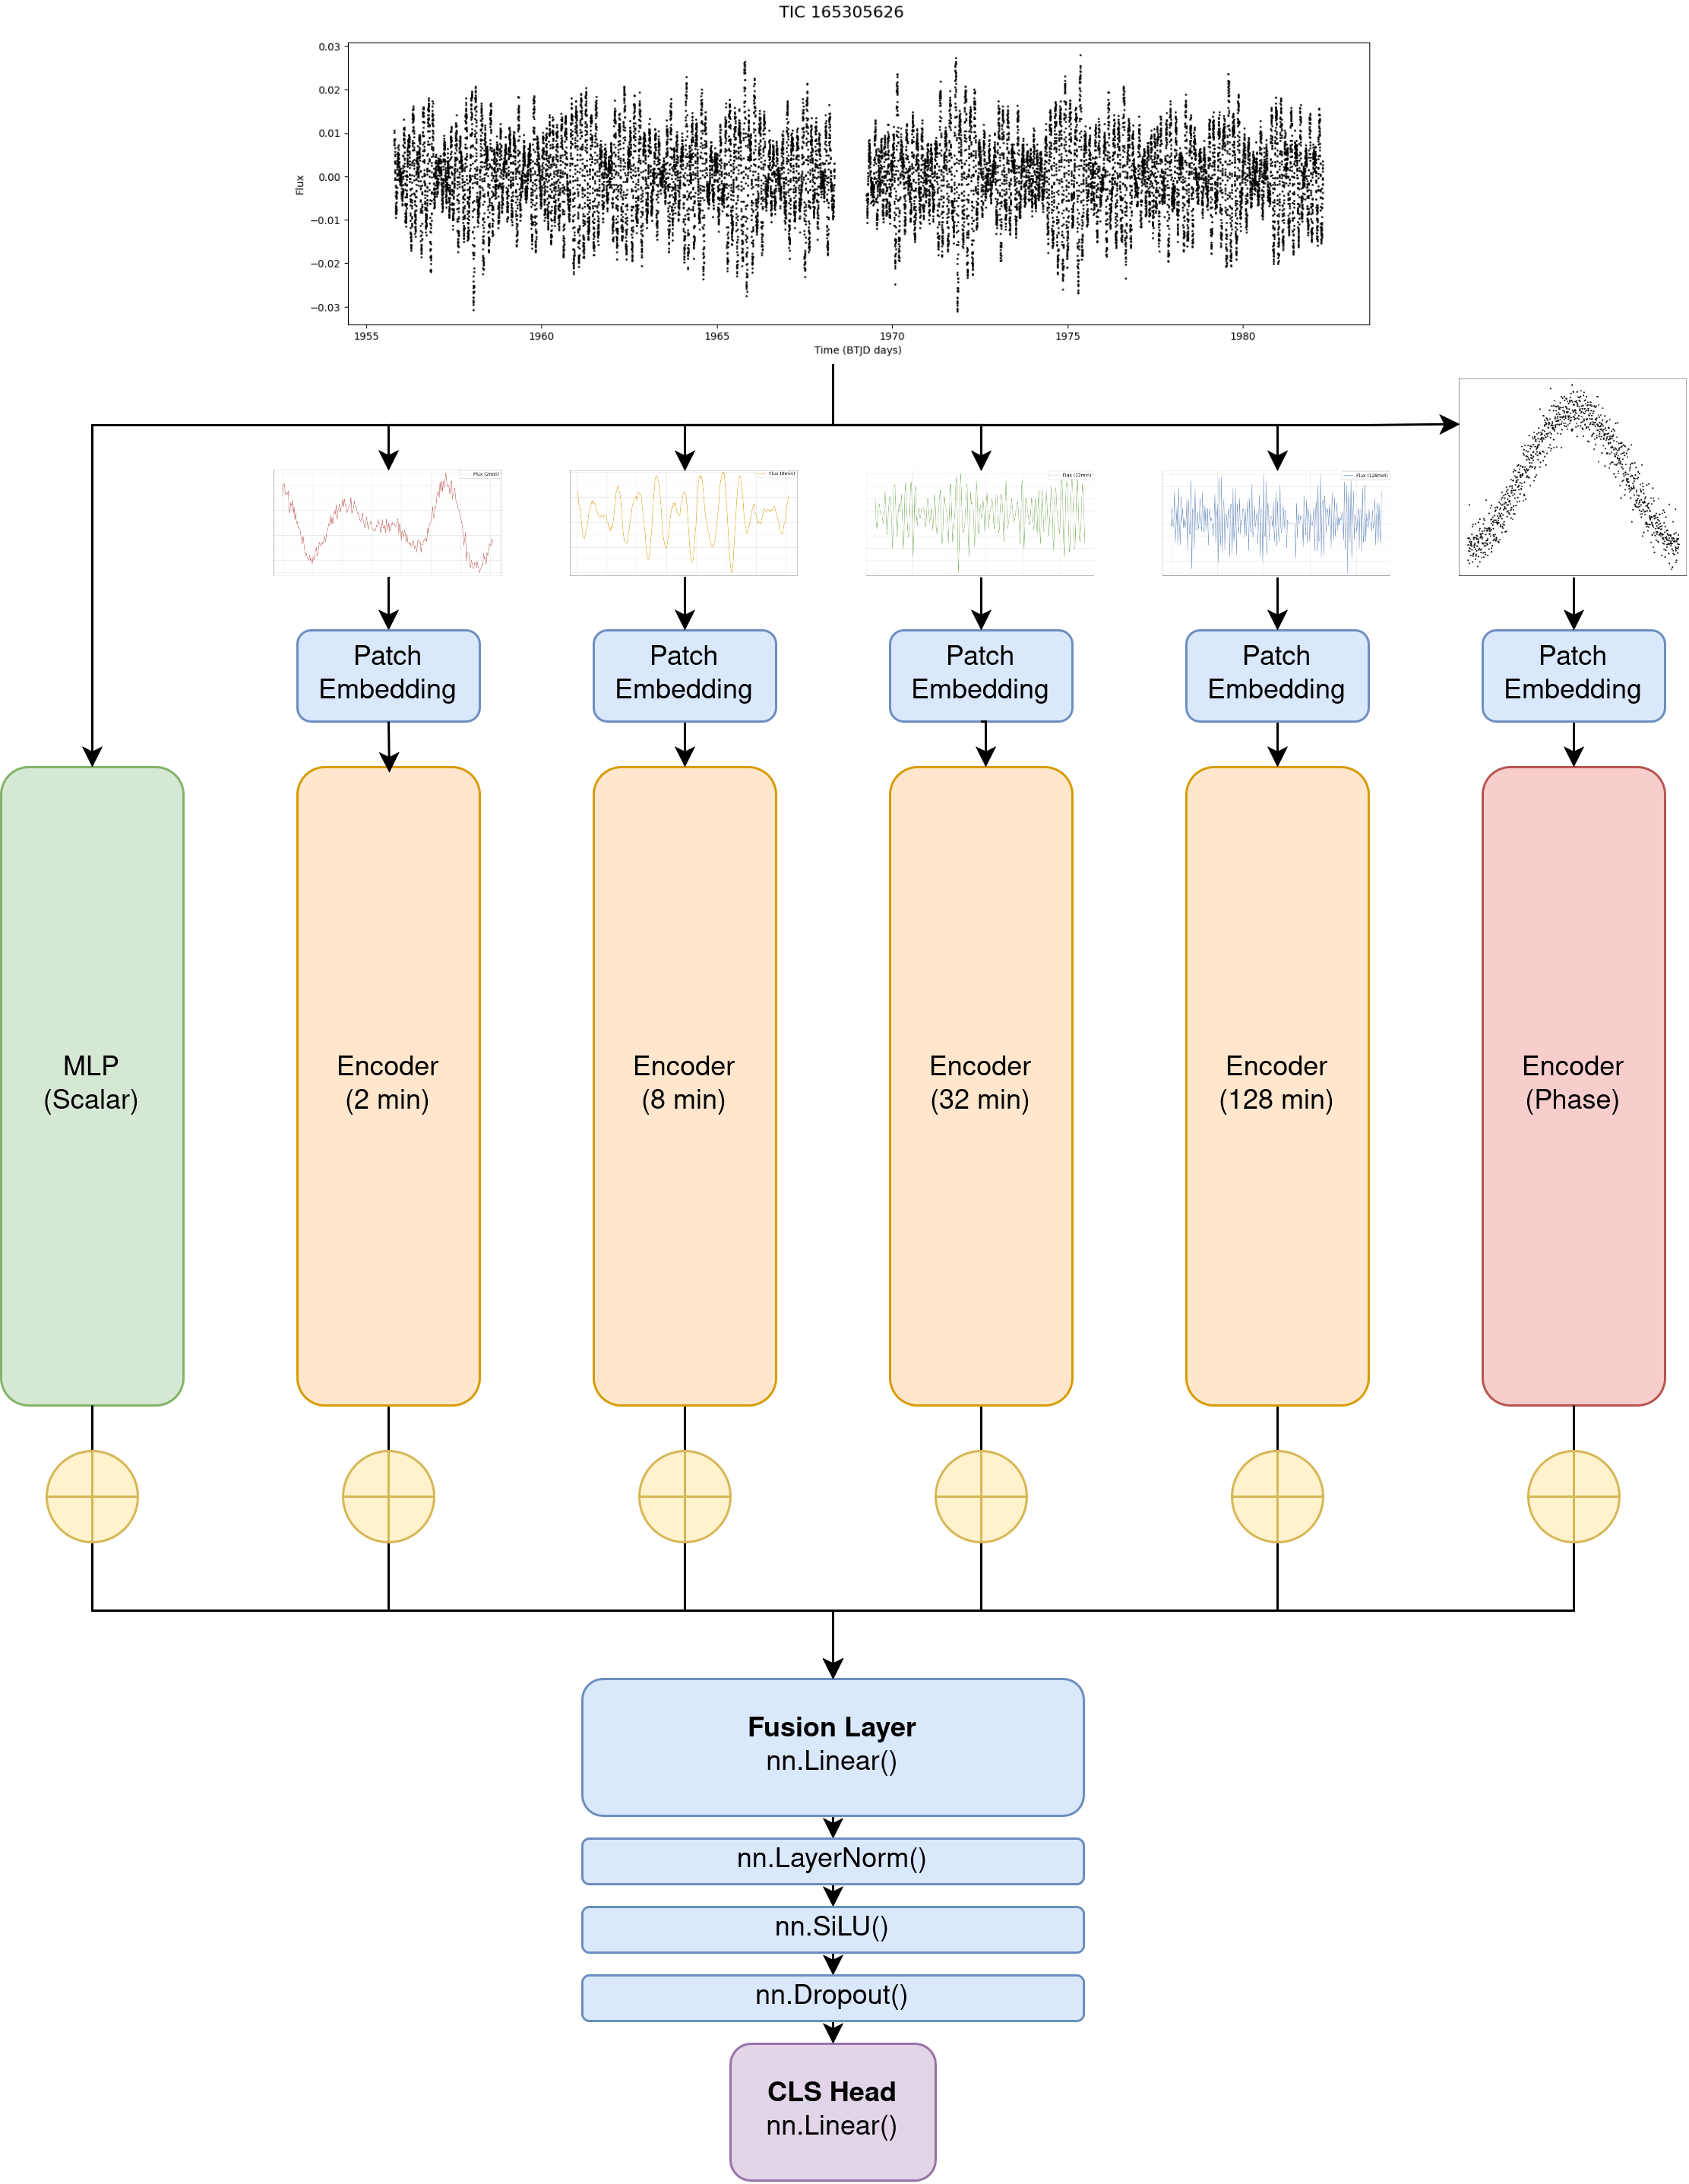
\includegraphics[width=0.92\textwidth]{model_architecture.png}
        \caption{Multi-branch architecture. Each of the five sequence channels is processed by a
        separate encoder-only transformer branch; scalar features pass through a small MLP. The
        branch representations are combined by a linear fusion layer before classification. Any
        branch can be disabled, allowing arbitrary channel combinations to be tested under an
        otherwise identical configuration.}
        \label{fig:arch}
    \end{figure*}

    \subsection{Statistical patch embeddings}

    Per-point learnable embeddings were tested first, but overfitted readily and made
    attention costly, since every flux measurement becomes a token. We therefore use patch
    embeddings, augmented with summary statistics computed from each patch.

    An input tensor of shape $(L, D)$, where $L$ is the view length and $D$ the number of
    input channels ($\Phi$ and $\Phi_{\mathrm{err}}$), is reshaped to $(N, P, D)$ for patch
    size $P$ and $N = L/P$ patches, padding as required. For each patch $j$ and channel $d$
    we compute, using only valid positions according to the mask, the mean $\mu_{j,d}$, the
    standard deviation $\sigma_{j,d}$, the minimum, the maximum, and the slope, approximated
    as $\mathrm{cov}(\Phi, t)/\mathrm{var}(t)$; a single additional scalar records the
    fraction of valid points in the patch. The resulting vector of length $5D+1$ is projected
    to $d_{\mathrm{model}}$ by a two-layer MLP. Relative to raw-flux patch embeddings, this
    representation improved macro $F_1$ by $0.05$--$0.10$, the single largest architectural
    gain we measured.

    \subsection{Segment- and class-weighted loss}
    \label{sec:loss}

    Training minimises a segment-level cross-entropy in which class weights correct for class
    imbalance and a per-segment weight prevents objects with many segments from dominating.
    For segment $i$ belonging to object $t$ with $n_t$ segments, the segment weight is
    $s_i = 1/n_t$, and the batch loss is
    \begin{equation}
        \mathcal{L} = \frac{\sum_{i=1}^{B} s_i\, L^{(i)}_{\mathrm{WCE}}}
        {\sum_{i=1}^{B} s_i} ,
        \label{eq:loss}
    \end{equation}
    where $B$ is the batch size and $L^{(i)}_{\mathrm{WCE}}$ is the class-weighted
    cross-entropy of segment $i$. The objective remains segment-based, but every object
    contributes approximately equally.

    \subsection{Object-level aggregation and metrics}
    \label{sec:ticmetrics}

    The scientific target is the classification of a star, not of a 23-day window of its
    light curve. For each segment $i$ of object $t$ the model produces logits
    $\mathbf{z}_{t,i}$ over $C$ classes, which are converted to probabilities by a softmax and
    averaged over the $n_t$ segments,
    \begin{equation}
        \bar{p}_{t,c} = \frac{1}{n_t}\sum_{i=1}^{n_t}
        \mathrm{softmax}\!\left(\mathbf{z}_{t,i}\right)_c ,
        \qquad
        \hat{y}_t = \arg\max_c\, \bar{p}_{t,c} .
        \label{eq:agg}
    \end{equation}
    This yields exactly one prediction per object, from which TIC-level accuracy and macro
    $F_1$ are computed. Figure~\ref{fig:segtic} illustrates why the aggregation matters: an
    individual segment of an eclipsing binary may lack a clear secondary eclipse and be
    misclassified, while the probability average over all segments remains correct.

    We report both segment-level and TIC-level metrics, but use TIC-level macro $F_1$ on the
    validation set as the sole criterion for checkpoint selection, since it corresponds
    directly to the way the model would be applied to unlabelled data.

    \begin{figure}[!t]
        \centering
        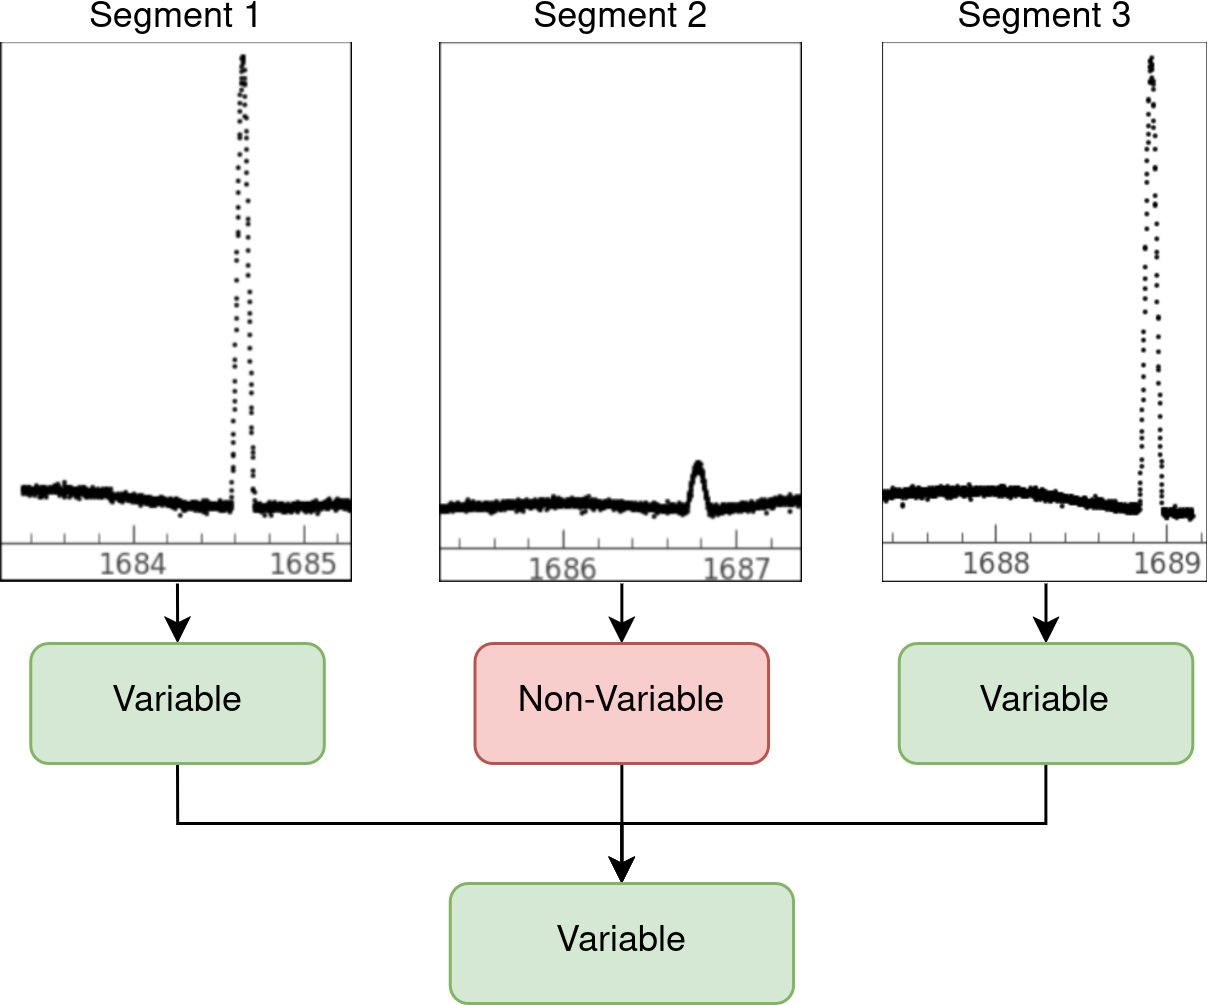
\includegraphics[width=\columnwidth]{segment_vs_tic_classification.png}
        \caption{Segment-level versus object-level classification. One of the three segments of
        this eclipsing binary is misclassified as non-variable because its secondary eclipse is
        poorly defined; averaging class probabilities over segments recovers the correct label.}
        \label{fig:segtic}
    \end{figure}

    \subsection{Backbones}

    Three backbones are supported within the same architecture:

    \begin{description}
        \item[Transformer] Standard encoder blocks trained from scratch, implemented in PyTorch
        \citep{Paszke2019}.
        \item[Chronos-2] A 120M-parameter encoder-only time series foundation model developed by
        Amazon \citep{Ansari2025}. It was pretrained for probabilistic forecasting on
        generic time series and performs its own tokenisation and patching, so it consumes
        the raw normalised flux.
        \item[Qwen\,2.5 0.5B] A 500M-parameter pretrained large language model
        \citep{Qwen2025}, adapted to accept patch embeddings in place of text tokens.
    \end{description}

    We did not evaluate pretrained vision transformers, since the problem is one-dimensional
    at the physical level and rendering light curves as images discards information for no
    obvious benefit.

    Both pretrained backbones were adapted with LoRA \citep{Hu2021}, with the original
    weights frozen and rank-8 adapters ($\alpha = 16$) trained alongside the embedding,
    fusion, and classification heads.

    \subsection{Training protocol}

    A standard train/validation/test split at the TIC level was used, with the test set
    touched only once, for the final model. We also implemented $k$-fold cross-validation,
    but it multiplied training time by $\sim k$ without a measurable improvement in
    validation performance, so it was not adopted.

    Hyperparameters were fixed after an initial exploration phase and held constant across
    all comparisons (Table~\ref{tab:hyper}). Patch size proved the most influential single
    parameter: values from 4 to 64 were tested, and 16 was clearly optimal, with much larger
    or smaller values either overfitting or failing to converge. The transformer width
    parameters showed a threshold behaviour -- below a minimum viable value the model does
    not converge, above it further capacity brings no gain. Cosine annealing of the learning
    rate outperformed both a flat schedule and the other schedulers tested. Balanced
    sampling, tried on the imbalanced Task~B, caused over-prediction of the eclipsing class
    and was abandoned in favour of the weighting in Eq.~(\ref{eq:loss}).

    \begin{table}[!t]
        \caption{Training configuration. Values in parentheses apply to the fine-tuned models.}
        \label{tab:hyper}
        \centering
        \small
        \begin{tabular}{ll}
            \toprule
            Parameter             & Value                                          \\
            \midrule
            Epochs                & 50 (10 for fine-tunes)                         \\
            Learning rate         & $5\times10^{-5}$, cosine annealed to $10^{-6}$ \\
            Optimiser             & AdamW                                          \\
            Weight decay          & $1\times10^{-2}$                               \\
            Batch size            & 64 (32 for Qwen\,2.5)                          \\
            Patch size            & 16 (Chronos-2 consumes raw flux)               \\
            Dropout               & 0.15                                           \\
            $n_{\mathrm{head}}$   & 8                                              \\
            $n_{\mathrm{layers}}$ & 4                                              \\
            $d_{\mathrm{model}}$  & 256                                            \\
            $d_{\mathrm{ff}}$     & 1024                                           \\
            $d_{\mathrm{fusion}}$ & 256                                            \\
            LoRA $r$ / $\alpha$   & 8 / 16                                         \\
            Loss                  & Eq.~(\ref{eq:loss})                            \\
            \bottomrule
        \end{tabular}
    \end{table}

%-----------------------------------------------------------------------


    \section{Results}
    \label{sec:results}

    \subsection{Experiment overview}

    Sixteen configurations were trained on both tasks under the protocol of
    Sect.~\ref{sec:method}. The baseline replaces the transformer blocks with two 1D
    convolutional layers (kernel size 3) while keeping the multi-branch architecture,
    preprocessing, loss, and aggregation identical, so that the comparison isolates the
    sequence encoder. Table~\ref{tab:summary} lists validation TIC-level macro $F_1$ for all
    configurations.

    \begin{table}[!t]
        \caption{Validation TIC-level macro $F_1$ for all evaluated configurations. The best
        result per task is in bold.}
        \label{tab:summary}
        \centering
        \small
        \begin{tabular}{llcc}
            \toprule
            Model          & Backbone       & Task A          & Task B          \\
            \midrule
            Baseline       & CNN            & 0.9061          & 0.9232          \\
            \midrule
            2-min view     & Transformer    & 0.8396          & 0.6618          \\
            8-min view     & Transformer    & 0.8704          & 0.8223          \\
            32-min view    & Transformer    & 0.8684          & 0.8614          \\
            128-min view   & Transformer    & 0.8436          & 0.9110          \\
            \midrule
            4-channel      & Transformer    & 0.8931          & 0.9230          \\
            6-channel      & Transformer    & 0.8983          & 0.9240          \\
            \midrule
            Chronos-2      & TSFM fine-tune & \textbf{0.9261} & \textbf{0.9496} \\
            Qwen\,2.5 0.5B & LLM fine-tune  & 0.9129          & 0.9139          \\
            \bottomrule
        \end{tabular}
    \end{table}

    Three results stand out. First, single-view transformers are consistently worse than the
    baseline, and the ranking of views is task-dependent in exactly the way the physics
    predicts: the 2-min view is competitive on Task~A but collapses on Task~B
    ($F_1 = 0.66$), because separating rotating from eclipsing variables requires timescales
    of days, which a 8.5-hour window cannot resolve. Conversely the 128-min view is the best
    single view on Task~B and among the worst on Task~A.

    Second, combining views recovers most of the gap: the 4- and 6-channel transformers reach
    the baseline on Task~B and come close on Task~A. Since the baseline CNN has access to the
    same six channels, the small residual difference indicates that the multi-resolution
    representation and the segmentation scheme -- not the choice of sequence encoder --
    account for most of the achievable performance.

    Third, the fine-tuned Chronos-2 model is the only configuration that exceeds the baseline
    on both tasks, by $\Delta F_1 = 0.020$ and $0.026$ respectively. The fine-tuned LLM
    outperforms every from-scratch transformer on Task~A but does not beat the baseline on
    either task, despite being four times larger than Chronos-2 -- consistent with the
    expectation that pretraining on time series transfers better to photometric data than
    pretraining on text.

    We attempted to improve on Chronos-2 by further tuning: increasing dropout, varying the
    LoRA rank and scaling, testing additional channel combinations, and enlarging the fusion
    head. None of these produced a configuration better than the original, which was
    therefore adopted as final. Training took approximately 100\,min (Task~A) and 30\,min
    (Task~B). The checkpoints selected by validation TIC-level macro $F_1$ were epoch 5 for
    Task~A and epoch 4 for Task~B (Fig.~\ref{fig:curves}); in both cases the validation loss
    had not yet begun to rise and the training loss was only marginally lower, indicating
    that the selected checkpoints are not significantly overfitted.

    \begin{figure*}[!t]
        \centering
        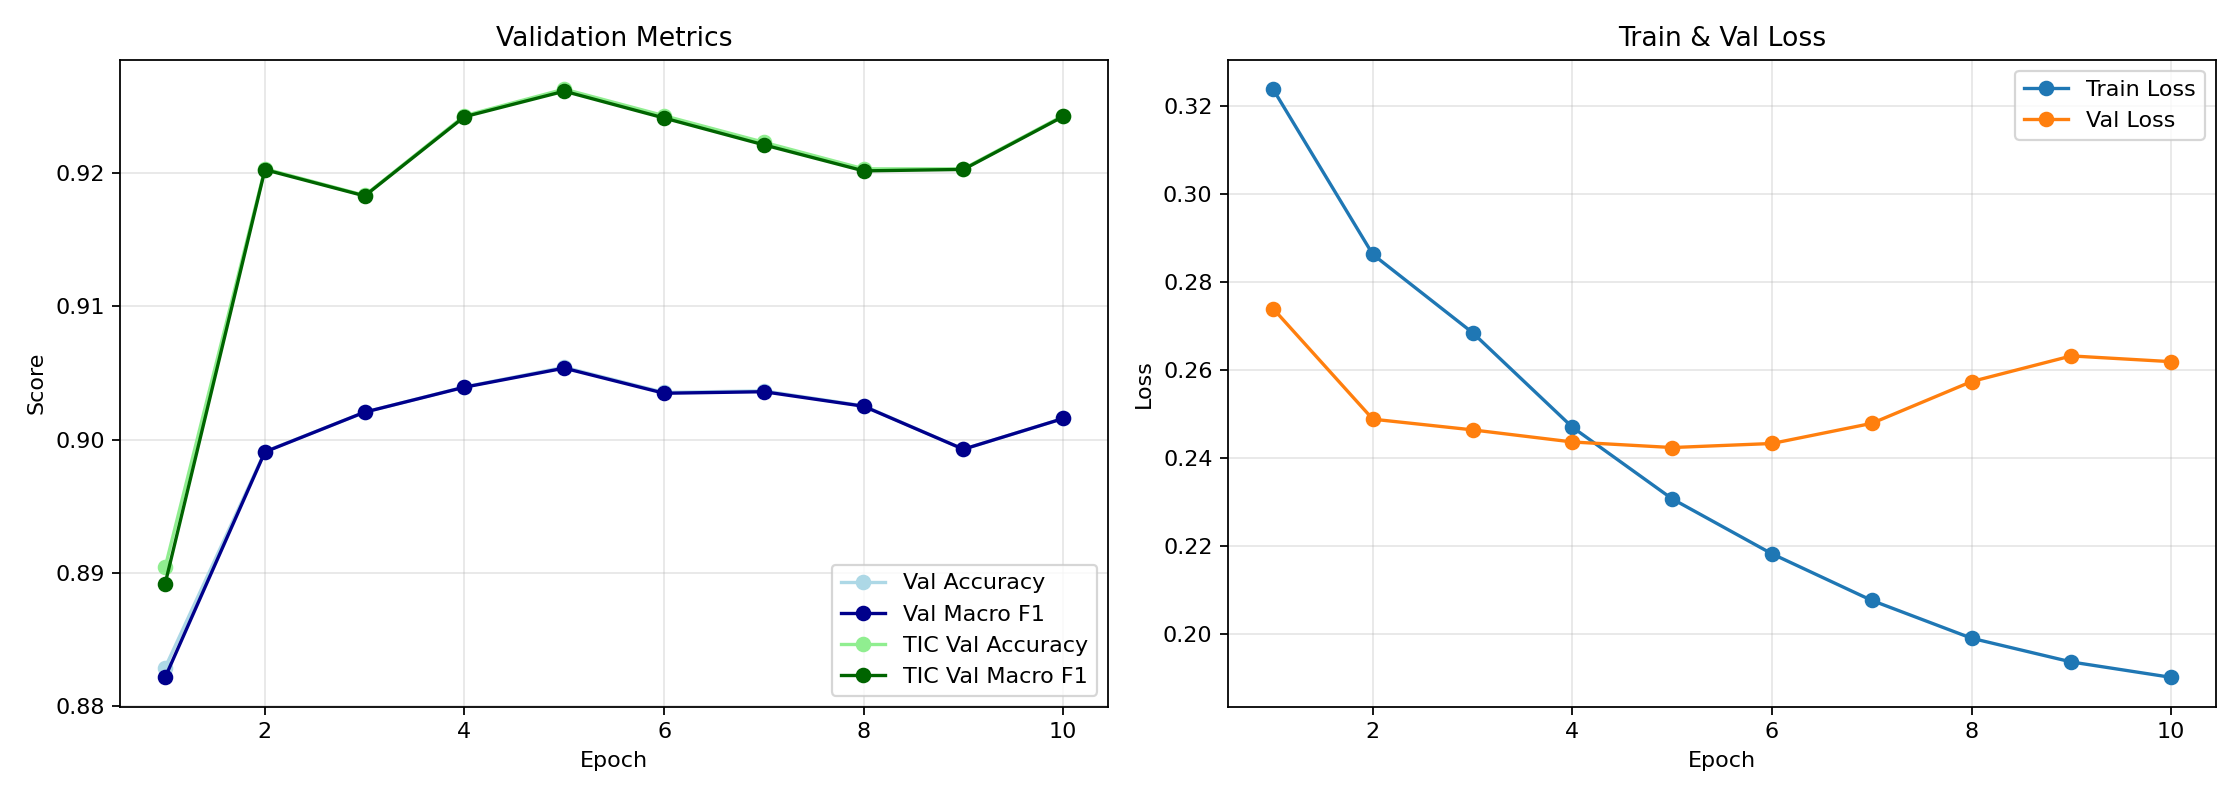
\includegraphics[width=0.49\textwidth]{phase3_A_chronos_training_curves.png}
        \hfill
        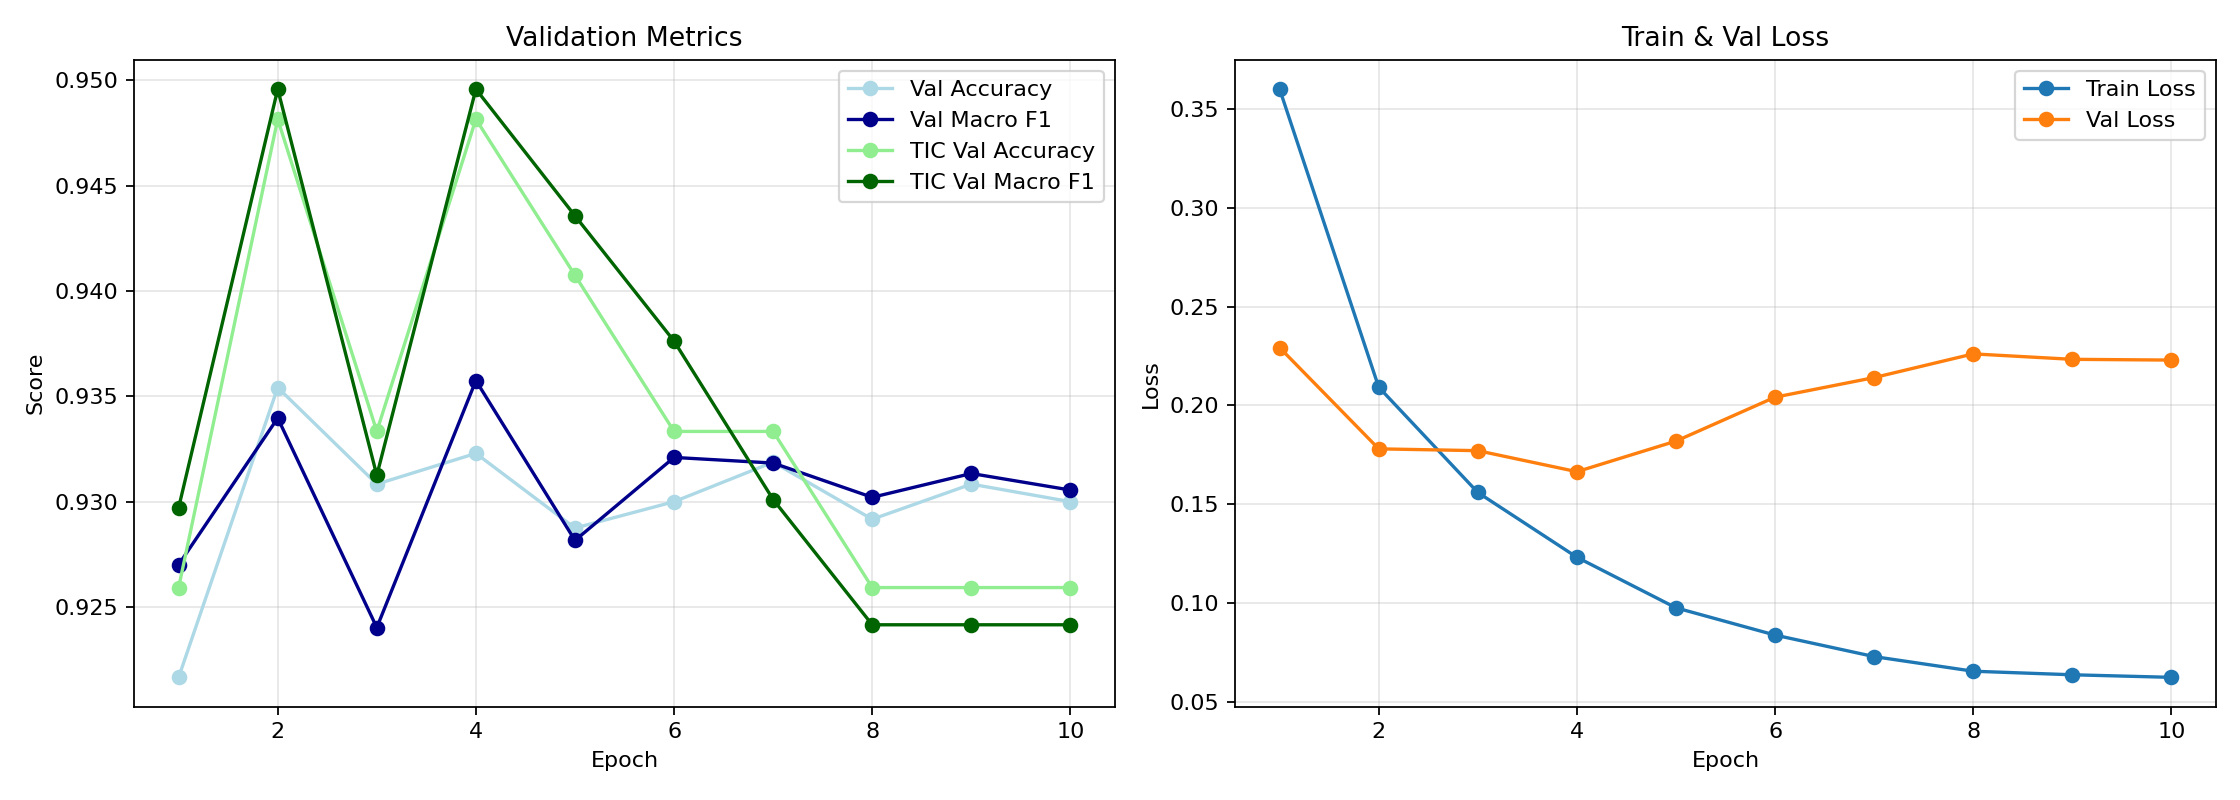
\includegraphics[width=0.49\textwidth]{phase3_B_chronos_training_curves.png}
        \caption{Training and validation curves of the fine-tuned Chronos-2 model for Task~A
            (left) and Task~B (right). The selected checkpoints are epoch 5 and epoch 4
            respectively, just before the validation loss begins to diverge from the training loss.}
        \label{fig:curves}
    \end{figure*}

    \subsection{Test-set performance}

    Table~\ref{tab:test} reports the performance of the final model on the held-out test set,
    which was used exactly once.

    \begin{table}[!t]
        \caption{Test-set performance of the fine-tuned Chronos-2 model.}
        \label{tab:test}
        \centering
        \small
        \begin{tabular}{lcccc}
            \toprule
            \multicolumn{5}{l}{\textbf{Task A} -- accuracy 0.870, macro $F_1$ 0.869,} \\
            \multicolumn{5}{l}{\phantom{\textbf{Task A} -- }TIC accuracy 0.895, TIC macro $F_1$ 0.893} \\
            \midrule
            Class            & Precision & Recall & $F_1$ & Support \\
            \midrule
            N (non-variable) & 0.85      & 0.97   & 0.90  & 259     \\
            V (variable)     & 0.96      & 0.82   & 0.88  & 243     \\
            \midrule
            \multicolumn{5}{l}{\textbf{Task B} -- accuracy 0.900, macro $F_1$ 0.834,} \\
            \multicolumn{5}{l}{\phantom{\textbf{Task B} -- }TIC accuracy 0.933, TIC macro $F_1$ 0.880} \\
            \midrule
            Class            & Precision & Recall & $F_1$ & Support \\
            \midrule
            E (eclipsing)    & 0.83      & 0.67   & 0.74  & 15      \\
            P (pulsating)    & 0.94      & 0.99   & 0.96  & 81      \\
            R (rotating)     & 0.94      & 0.93   & 0.94  & 39      \\
            \bottomrule
        \end{tabular}
    \end{table}

    On Task~A the TIC-level macro $F_1$ drops by $\approx 0.02$ relative to validation, which
    is a reasonable generalisation gap for a dataset of this size. The composition of the
    score changes, however: for the variable class, precision rises and recall falls
    substantially compared with validation. The classifier has become conservative.

    On Task~B the drop is larger, $\Delta F_1 \approx 0.07$. It is almost entirely
    attributable to the eclipsing class, whose recall of 0.67 corresponds to five
    misclassified objects out of fifteen. The pulsating and rotating classes generalise
    essentially without loss, with test metrics within $0.01$ of their validation values.

%-----------------------------------------------------------------------


    \section{Discussion}
    \label{sec:discussion}

    \subsection{Failure modes}

    We inspected each of the five misclassified eclipsing systems individually
    (Table~\ref{tab:misclass}). Every one is an atypical member of its class. Two are ELL
    systems whose ellipsoidal maxima are smooth rather than sharp, making them
    morphologically indistinguishable from spotted rotating variables at the available
    signal-to-noise; one EW system has a continuously varying light curve resembling a
    pulsator; one EA system is too noisy for its eclipses to be recovered; and one EA system
    has an atypically long period, eclipsing roughly once per 50\,d, so that most 23-day
    segments contain no eclipse at all (Fig.~\ref{fig:longperiod}).

    \begin{table}[!t]
        \caption{The five misclassified eclipsing systems in the Task~B test set.}
        \label{tab:misclass}
        \centering
        \small
        \begin{tabular}{llp{4.2cm}}
            \toprule
            TIC       & Subtype & Remark                                               \\
            \midrule
            224595426 & EA      & Very noisy; eclipses not clearly identifiable.       \\
            229710150 & ELL     & Smooth maxima; resembles a rotating variable.        \\
            259238257 & ELL     & Smooth maxima; resembles a rotating variable.        \\
            288346083 & EA      & Atypically long period, one eclipse per $\sim$50\,d. \\
            362226108 & EW      & Continuous variation resembling a pulsator.          \\
            \bottomrule
        \end{tabular}
    \end{table}

    \begin{figure}[!t]
        \centering
        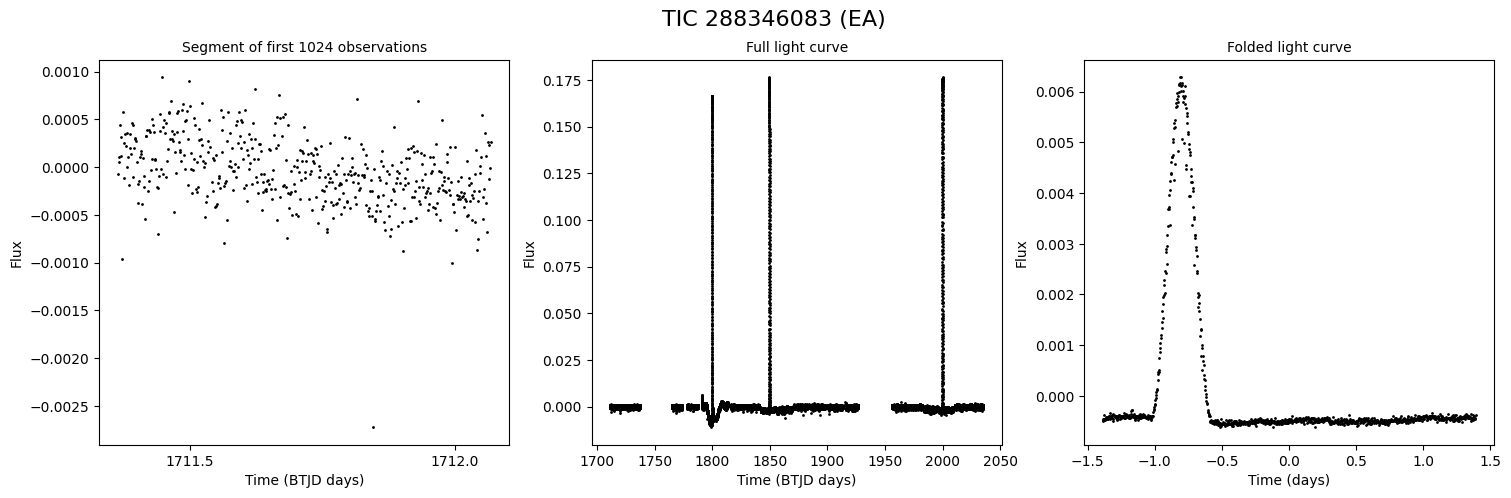
\includegraphics[width=\columnwidth]{long_period_star.png}
        \caption{TIC 288346083, a misclassified EA system with an atypically long period. Most
        segments contain no eclipse, so the object-level probability average is dominated by
        featureless windows.}
        \label{fig:longperiod}
    \end{figure}

    The last case exposes a structural limitation of segment-based aggregation by mean
    probability: for objects whose defining feature occurs in a small minority of segments,
    averaging dilutes the signal. A max-probability or attention-weighted aggregation would
    address this, at the cost of increased sensitivity to single-segment false positives.
    The two ELL cases are a different matter -- the distinction between ellipsoidal variation
    and rotational modulation is genuinely marginal from photometry alone and would challenge
    a human classifier as well.

    \subsection{Operating point}

    The precision--recall asymmetry on Task~A has practical consequences. A classifier with
    0.96 precision and 0.82 recall on the variable class is well suited to building large,
    high-purity samples of variable stars from unlabelled archives -- for instance as a
    corpus for unsupervised pretraining -- but will miss roughly one variable in five. For
    applications where completeness matters more than purity, the decision threshold on
    $\bar{p}_{t,c}$ should be adjusted accordingly; the aggregation of Eq.~(\ref{eq:agg})
    provides a calibrated probability at which to do so.

    \subsection{Throughput}

    Survey-scale application requires the pipeline to process $\sim 10^6$ light curves in
    reasonable time. There are two potential bottlenecks. Preprocessing runs at
    $\approx 13.8$ light curves\,s$^{-1}$ on an 8-core AMD Ryzen 5 9700X, i.e. about
    $1.2\times10^6$ per day; inference on the fine-tuned Chronos-2 model runs at
    $\approx 12.6$ light curves\,s$^{-1}$ on a consumer AMD Radeon RX\,9070 GPU, about
    $1.1\times10^6$ per day. The two stages are therefore well balanced, and the complete
    pipeline can process a million light curves per day on a single consumer workstation.
    Neither figure reflects a tuned implementation; datacentre GPUs and wider parallelism
    would improve both substantially.

    \subsection{Applicability}

    This work forms part of an ongoing effort at the Astronomical Institute of the Czech
    Academy of Sciences to build automated classifiers for the identification of interesting
    objects, exoplanets in particular. Existing transit-search pipelines produce large
    numbers of false positives, typically variable stars misidentified as planet hosts.
    Because transits resemble the eclipses of a detached binary far more than they resemble
    pulsation or rotational modulation, a Task~B classifier that reliably recognises
    pulsating and rotating variables can remove a substantial fraction of these false
    positives before human vetting.

    The timing is favourable: Gaia DR4 \citep{Prusti2016} and PLATO \citep{Rauer2025} will
    both deliver large volumes of photometric time series in the near future. Models of the
    kind presented here can either contribute directly to their filtering or serve as a
    starting point for survey-specific classifiers.

    \subsection{Limitations and outlook}

    The principal limitation is the size of the labelled sample, and in particular the 101
    eclipsing systems, which is what ultimately bounds Task~B performance. Three directions
    follow naturally. First, unsupervised pretraining on the millions of available unlabelled
    TESS light curves would let the model learn the structure of photometric time series
    without labels -- the domain gap that Chronos-2 must currently bridge from generic time
    series. Second, modern architectural components -- gated feed-forward networks,
    FFT-based attention, and learned rather than linear fusion, including gating at the
    branch level -- are straightforward additions to the present design. Third, and most
    directly, a larger labelled catalogue, particularly of eclipsing systems, would help more
    than any architectural change.

%-----------------------------------------------------------------------


    \section{Conclusions}
    \label{sec:conclusions}

    We have evaluated transformer-based classifiers of stellar variability on 3347 manually
    labelled TESS light curves, comparing transformers trained from scratch, fine-tuned
    pretrained models, and a convolutional baseline under an identical protocol. Our main
    findings are:

    \begin{enumerate}
        \item Representing each light-curve segment by multiple time-domain views at different
        cadences is the decisive design choice. Single-view transformers underperform the
        baseline on both tasks, and the failure is systematic: high-cadence views cannot
        resolve day-scale morphology and low-cadence views cannot resolve pulsation.
        Combining four views closes most of the gap.
        \item Fine-tuning a time series foundation model transfers effectively to astronomical
        photometry. Chronos-2 with LoRA adapters was the only configuration to beat the
        convolutional baseline on both tasks, reaching validation TIC-level macro $F_1$ of
        0.926 and 0.950, and test values of 0.893 and 0.880.
        \item Pretraining domain matters more than model size. The 500M-parameter LLM did not
        match the 120M-parameter TSFM, despite being four times larger.
        \item Statistical patch embeddings, which augment each patch with its mean, dispersion,
        extrema, slope, and valid fraction, were worth $0.05$--$0.10$ in macro $F_1$ -- the
        largest single architectural gain we measured.
        \item The residual errors are dominated by genuinely atypical objects. All five
        misclassified eclipsing systems in the test set are non-standard, and two of them
        are arguably ambiguous from photometry alone.
    \end{enumerate}

    The complete pipeline sustains $\sim10^6$ light curves per day on a single consumer
    workstation, which makes it directly applicable to survey-scale archives and to the
    reduction of false positives in transit searches, ahead of the Gaia DR4 and PLATO data
    releases.

    \begin{acknowledgements}
% TODO: complete before submission -- funding, grant numbers, institutional support.
        We thank M. Skarka for providing the cleaned labelled dataset. This paper includes data
        collected by the TESS mission, obtained from the Mikulski Archive for Space Telescopes
        (MAST). Funding for the TESS mission is provided by the NASA Explorer Program.
    \end{acknowledgements}

%-----------------------------------------------------------------------


    \section*{Data availability}

% TODO: replace with the DOI of the archived release before submission.
    The training code, configuration files, and experiment logs are available at
    \url{https://github.com/}. The labelled catalogue is published by \citet{Skarka2022};
    the underlying TESS light curves are publicly available from MAST.

%-----------------------------------------------------------------------
    \bibliographystyle{aa}
    \bibliography{references}

\end{document}
